
% This chapter presents the implementation of a distributed system running on Matrix and developed with Paragon as described in the criterias.

This chapter describes the implementation of the prototype in the case study. The prototype is a system for sending and retrieving patient journals among different hospitals. The system relies on Matrix as the secure communication channel and storage.


\section{Journal system}

% Describe the requirements for the journal system.
A journal system serves an important purpose by providing patient journals to different hospitals and clinics. If a patient arrives at the ER and the doctor cannot access the patient's journal then the treatment of the patient gets problematic. A doctor might miss out on important details about the patient or even worse prescribe medication that might give the patient an allergic reaction. The availability of a patient journal is a necessity however the number of medical employees that have access to such a journal has raised privacy concerns. Around 90.000 medical employees have access to patient journals. Consider the scenario where a patient gets referred to a physiotherapist with muscle pain. When the therapist opens the journal the full medical history will be present; if the patient had received psychiatric treatment those session would be readable too. Furthermore a patient journal is accessible by a large number of unrelated medical employees with the only prevention mechanism being logging and audit trails.


The lack of secure information flow is evident and the prototype demonstrates how Information-Flow control can be leveraged to enforce security policies concerning the information. The journal system is a small distributed system where Hospitals can send, receive and store patient journals. Matrix provides the distributed structure and is responsible for securely storing and transmitting the journals. Paragon provides secure information flow at the endpoints hence providing end-to-end security. 
The following requirements are defined for the prototype:

\begin{itemize}
	\item A patient journal contains high (secret) and low (public) information.
	\item A patient journal is send and received securely over a channel.
	%\item A patient journal can only be appended to. 
	\item Hospitals have shared access to patient journals. 
	\item A hospital has two actors: Doctor and Secretary.
	\item A doctor must have the patient in care to access the high information in a journal.
	\item The doctor can see the full patient journal.
	\item The doctor can add to secret fields of a patient journal.
	%\item The secretary must work under the Doctor who has the patient in care to access it.
	\item A secretary can only see some parts of the journal.
	\item A secretary can edit the public parts of a journal.
\end{itemize}

The following non-functional requirements are defined:

\begin{itemize}
	\item Confidentiality: the system must ensure the confidentiality throughout the system according to the security policies at all times.
	\item Integrity: the system must ensure that only intended actors can modify the specific parts of a patient journal.
	\item Accessibility: the system can only used from the hospital hence retrieving patient journals outside the hospital is not possible.
\end{itemize}


\subsection{System design}


The system consists of two components; \emph{Matrix} and the \emph{client}. The Matrix component encapsulates the Matrix SDK and provides an interface. The client component consumes that interface and can be considered as the endpoint in a communication channel. The client component provides secure information flow for data received through Matrix. 
The component diagram in figure \ref{fig:matrix_component} depicts this.

\begin{figure}[H] 
	\hspace*{-1cm}
	\centering
	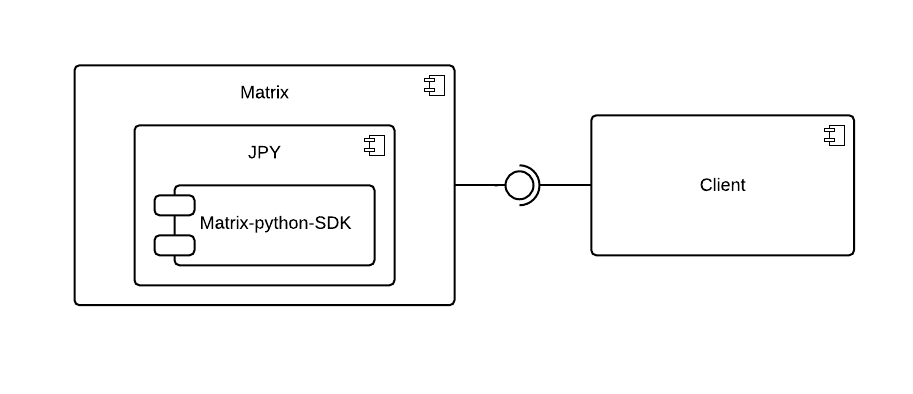
\includegraphics[width=14cm]{figures/matrix_component.png}
	\caption{Component diagram for the system}
	\label{fig:matrix_component}
\end{figure}

Matrix provides several SDK libraries that client application can be build on top of. The most prominent is the Javascript Matrix SDK. It is the best maintained with the largest feature set however it is not compatible with the Java based Information-Flow Control tool Paragon. A Java Matrix SDK exists but it is an early alpha version with end-to-end encryption not implemented yet. The Python Matrix SDK is another major SDK with support for end-to-end encryption in beta. The Python Matrix SDK is used in the Matrix component through a Java-Python bridge \emph{JPY} that can embed Python code in Java as shown in the Matrix component in figure \ref{fig:matrix_component} 


\subsubsection{Matrix}
%Matrix API's
% A lot of things are handled under the hood by the matrix SDK.
Matrix is an important component in the system. It manages the transmission and storage of patient journals through rooms while managing end-to-end encryption. The encryption mechanism is automatically provided and the SDK manages the session keys under the hood.  As described in section \ref{matrix:architecture} a room is a conceptual place for sending an receiving events and events can be any of any structure. The event history in a rooms is replicated at each homeserver. 

The following design choices and assumptions are made regarding Matrix and the system: 

\begin{itemize}
	\item A homeserver represents a hospital server that replicates the history of a patient journal. 
	\item A room represents a single patient journal's version history.
	\item An event represents a patient journal.  
	\item The latest event in a room is the global state of the patient journal.
	\item A hospital is represented by a single matrix user that participates in a room.
	\item A hospital's matrix user is used by doctors and secretaries to access patient journals. 
\end{itemize}


The room can be considerably large since many different types of hospitals needs access to a patient journal. This puts a lot of responsibility on securing the endpoints but also adds concern to who controls the rooms and how hospitals are added. A central authority would be managing all room whom all participants in the room trust. That authority would be the government which are responsible for creating and managing the rooms. Only the authority can invite and remove Hospitals from a room. Hospitals can only join a room if they have been invited. The rooms  


\subsubsection{Client}


 The hospital keeps track of all journals they have access to through a hashmap with key being the CPR and the value being the roomid. When a doctor or secretary want to retrieve a journal; the latest journal from the patient journal's room is fetched.
 he hospital retrieves the latest event 
 
 
 
The sessions between a doctor and a 

A patient journal the PatientJournal class depicts 

% Describe how the design with matrix would be
Figure \ref{fig:journalsystem} depicts the class diagram for the system.



\begin{figure}[H] 
	\hspace*{-1.3cm}
	\centering
	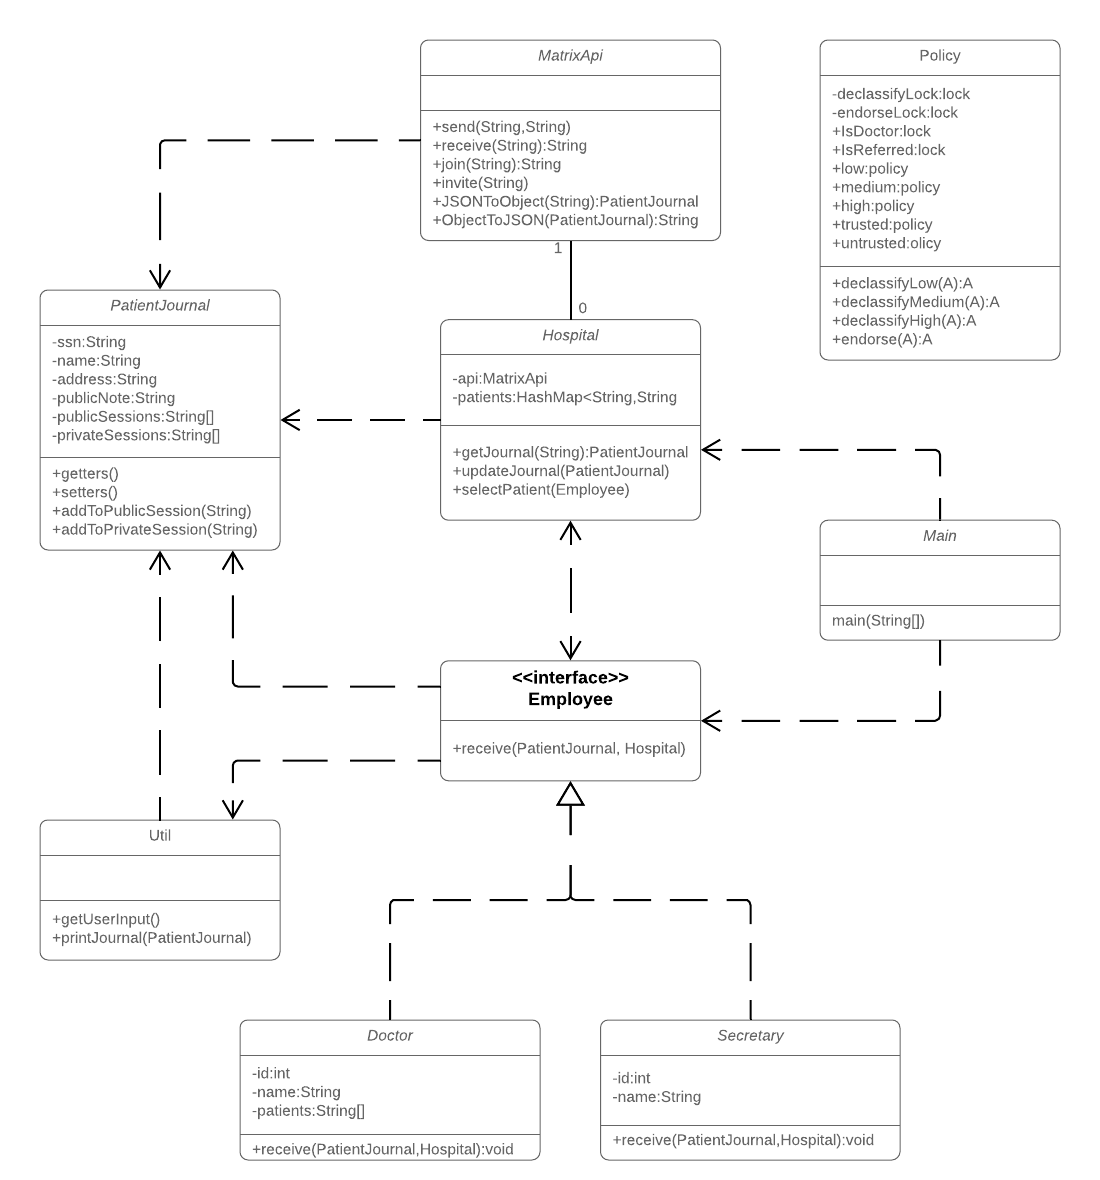
\includegraphics[width=14cm]{figures/journalsystem_class.png}
	\caption{Class diagram for the Journal system}
	\label{fig:journalsystem}
\end{figure}





\subsubsection{Limitations}

%Incompatibility with Paragon


A design problem is the concurrent writes to a journal from multiple hospital. Before writing to a journal; the latest version of the journal in Matrix is first retrieved and then the writes are appended to the journal. However multiple hospitals might have retrieved the latest journal and different doctors might have committed changes to the journal and send it to Matrix hence one of the writes would be lost since only the latest journal is retrieved. 

Another limitation is that the rooms a hospital can access are precreated and the hospitals in a room are preconfigured. 

%This is a common issue in distributed systems but is not handled in this solution. 


% It is assumed that a version control mechanism is in place and the latest journal received is always up to date.
% Solution merging data like version control systems like git.



\section{Paragon implementation}


\subsection{Policies and locks}

\subsubsection{Matrix API}

\subsubsection{Journal system}

%D Declaration examples

\subsubsection{Lattice}

\subsection{Declassification}

\subsection{Exception handling}


\subsection{Limitations}
 
%Technical requirements: -Msg type should be "m.text" when sending patient journal (JSON format). The convertion of string to JSON and vice versa should happen in the client.

\section{Summary}